\section{Configuration Table}
This section will describe what a configuration table is, and how our configuration table looks for the first sprint.

So what is a configuration table, you might ask?
A configuration table, is a table, with information about the project status. 
The table, will help you get a better overview of the solution you are trying to create, and why the problem needs to be solved.
Furethermore you can at all times see what the given sprint focus is, and when you need to review the solution, and other things, then you can just look at the configuration table, as one of the columns will be the criteria for the solution.

~\autoref{fig:example-configuration-table} shows the stucture of a configuration table.

\begin{figure}[]
    \centering
    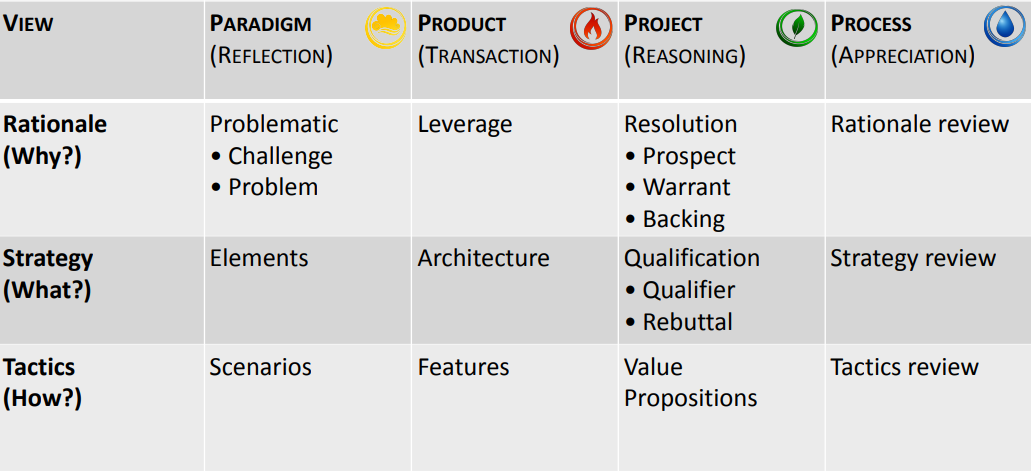
\includegraphics[width=\linewidth]{images/configurationTableExample.png}
    \caption{Structure of a Configuration table.}
    \label{fig:example-configuration-table}
\end{figure}

A configuration table consists of three areas, which is, \textbf{Rationale}, \textbf{Tactics} and \textbf{Strategy}.
Each of these have their own area of view in the given project, however, there are some elements which they share with oneanother.

\subsection{Rationale}
\subsection{Tactics}
\subsection{Strategy}


\begin{landscape}
    \begin{table}[]
        \tiny
    \begin{tabular}{|l|l|l|l|l|}
    \hline
    View & \multicolumn{1}{c|} {Paradigm} & \multicolumn{1}{c|} {Product} & \multicolumn{1}{c|}{Project} & Process \\ \hline
    Value & \multicolumn{1}{c|}{Reflection} & \multicolumn{1}{c|}{Transaction} & \multicolumn{1}{c|}{Reasoning} & Appreciation \\ \hline
    Rationale & \begin{tabular}[c]{@{}l@{}}Problematic:\\ \\ Challenge: Improve the communication \\ between customers and developers in \\ an Agile Software Development Process.\\ \\ Problem: The communication between \\ customers and developers are one of the \\ most challenging aspects of the \\ development process.\end{tabular} & \begin{tabular}[c]{@{}l@{}}Leverage:\\
        \begin{minipage} [t] {0.3\textwidth} 
            \begin{itemize}
            \item Docker
            \item Flutter
            \item DotNet
            \item Entity Framework
            \item PostgreSQL
            \item JavaScript Frameworks
           \end{itemize} 
          \end{minipage} 
    \end{tabular} & \begin{tabular}[c]{@{}l@{}}Resolution:\\ \\ Prospect: The communication \\ between developers and \\ product owners will become easy.\\ \\ Warrant: Because software \\ development is expensive, \\ and could reduce the \\ cost and increase the quality\\ \\ Backing: Inexpensive, \\ popular platform. Extensible\end{tabular} 
            & \begin{tabular}[c]{@{}l@{}}Criteria for resolution expectations:\\ 
                \begin{minipage} [t] {0.3\textwidth} 
                    \begin{itemize}
                    \item Is the problem still worth solving
                    \item Does the proposed solution solve the problem
                    \item Have we used the correct leverage points
                   \end{itemize} 
                  \end{minipage}    
                \\ \\ Findings:\end{tabular} \\ \hline
    Strategy  & \begin{tabular}[c]{@{}l@{}}Elements \& Ecology:\\ 
        \begin{minipage} [t] {0.35\textwidth} 
            \begin{itemize}
            \item The product owners problem domain will be visible
            \item The product owner will have more direct communication with the developers
            \item Making the development process transparent
           \end{itemize} 
          \end{minipage} 
    \end{tabular} & \begin{tabular}[c]{@{}l@{}}Architecture:\\ 
        \begin{minipage} [t] {0.2\textwidth} 
            \begin{itemize}
            \item Digital app editor module
            \item Digital issue tracking module
            \item Digital communication module
           \end{itemize} 
          \end{minipage}\end{tabular} & \begin{tabular}[c]{@{}l@{}}Qualification:\\ \\ Qualifier: Requires some \\ knowledge about using apps\\ \\ Rebuttal: Most people \\ have this skill\end{tabular} 
            & \begin{tabular}[c]{@{}l@{}}Criteria for architecture expectations: \\
            \begin{minipage} [t] {0.3\textwidth} 
                \begin{itemize}
                \item Is the architecture feasible
                \item Is the product user-friendly
               \end{itemize} 
              \end{minipage} \\
\\ Findings:\end{tabular} \\ \hline
    Tactics   & \begin{tabular}[c]{@{}l@{}}Scenarios:\\ 
        \begin{minipage} [t] {0.3\textwidth} 
            \begin{itemize}
            \item Product owner used the system to create tasks for developers
            \item Developers can take tasks and solve them
            \item The Product owner can at any time see how a task is going and see the progress
           \end{itemize} 
          \end{minipage} 
         \end{tabular} & \begin{tabular}[c]{@{}l@{}}Features:\\ 
            \begin{minipage} [t] {0.3\textwidth} 
                \begin{itemize}
                \item App editor where the Product owner can make their requirements visible
                \item Translate App editor to developer requirements
                \item The Product owner can at any time see how a task is going and see the progress
               \end{itemize} 
              \end{minipage} 
    \end{tabular} & \begin{tabular}[c]{@{}l@{}}Value Propostions:\\
        \begin{minipage} [t] {0.3\textwidth} 
            \begin{itemize}
            \item Translate customer requirements to product requirements
           \end{itemize} 
          \end{minipage} 
         \end{tabular} & 
    \begin{tabular}[c]{@{}l@{}}Criteria for value propostions \\ expectations: \\
        \begin{minipage} [t] {0.3\textwidth} 
            \begin{itemize}
            \item Is the translation effective
           \end{itemize} 
          \end{minipage} 
         \\ \\ Findings:\end{tabular} \\ \hline
    \end{tabular}
    \caption{}
    \label{tab:my-table}
    \end{table}
\end{landscape}